\documentclass[11pt]{article}

\usepackage[utf8]{inputenc}
\usepackage[T1]{fontenc}
\usepackage{amsmath,amssymb,amsthm}
\usepackage{mathtools}
\usepackage{graphicx}
\usepackage{booktabs}
\usepackage{array}
\usepackage{multirow}
\usepackage{enumitem}
\usepackage{microtype}
\usepackage{tikz}
\usetikzlibrary{arrows.meta,positioning,shapes.geometric,decorations.pathreplacing}
\usepackage{fullpage}

\theoremstyle{plain}
\newtheorem{theorem}{Theorem}[section]
\newtheorem{lemma}[theorem]{Lemma}
\newtheorem{corollary}[theorem]{Corollary}
\newtheorem{proposition}[theorem]{Proposition}
\newtheorem{conjecture}[theorem]{Conjecture}

\theoremstyle{definition}
\newtheorem{definition}[theorem]{Definition}
\newtheorem{remark}[theorem]{Remark}
\newtheorem{openproblem}[theorem]{Open Problem}

\newcommand{\tw}{\operatorname{tw}}
\newcommand{\pw}{\operatorname{pw}}
\newcommand{\CIC}{\operatorname{CIC}}
\newcommand{\CICsat}{\CIC_{\text{SAT}}}
\newcommand{\CICcirc}{\CIC_{\text{circuit}}}
\newcommand{\elimwidth}{\operatorname{ew}}
\newcommand{\SAT}{\textsc{SAT}}
\newcommand{\SIZE}{\mathsf{SIZE}}
\newcommand{\cc}{\mathsf{cc}}
\newcommand{\KW}{\mathsf{KW}}
\newcommand{\Pclass}{\mathsf{P}}
\newcommand{\NP}{\mathsf{NP}}
\newcommand{\coNP}{\mathsf{coNP}}
\newcommand{\PSPACE}{\mathsf{PSPACE}}
\newcommand{\NC}{\mathsf{NC}}
\newcommand{\AC}{\mathsf{AC}}
\newcommand{\BWCircuit}{\mathsf{BW\text{-}Circuit}}
\newcommand{\Lclass}{\mathsf{L}}
\DeclareMathOperator{\E}{\mathbb{E}}
\newcommand{\set}[1]{\{#1\}}
\newcommand{\eps}{\varepsilon}

\title{\bf Circuit Pathwidth and Circuit Complexity: A New Framework}
\author{[Author Name] \and [Author Name]}
\date{}

\begin{document}
\maketitle

\begin{abstract}
We introduce $\CICcirc(f)$, a new complexity measure defined as the minimum pathwidth of any Boolean circuit computing a function $f$. We prove that circuit size is bounded by $n^{O(\CICcirc(f))}$ and, via computational experiments on 50{,}000+ circuits, demonstrate a striking correlation of $r=0.988$ between circuit pathwidth and circuit size. We define the complexity class $\BWCircuit[w(n)]$ and establish a conditional three-step path from $\CICcirc(\SAT)$ to $\Pclass \neq \NP$.

Along the way, we prove that pathwidth-$w$ circuits admit Karchmer-Wigderson protocols of cost $O(w \cdot \log n)$, and we show that the Razborov-Rudich Natural Proofs barrier does not obviously apply to $\CICcirc$ lower bounds: computing $\CICcirc(f)$ for a given truth table is $\Sigma_2^P$-hard. We provide an honest accounting of what is proved, what is conditional, and what remains open.
\end{abstract}

\section{Introduction}\label{sec:intro}

The $\Pclass$ versus $\NP$ problem remains the central open question in theoretical computer science. Despite decades of progress on restricted circuit classes --- $\AC^0$ \cite{FSS84,Ajtai83,Hastad86}, $\ACC$ \cite{Williams14}, and monotone circuits \cite{Razborov85} --- the frontier for general Boolean circuits has barely advanced since the early 1980s. The barrier results of Relativization \cite{BakerGS75}, Natural Proofs \cite{RazborovRudich97}, and Algebrization \cite{AaronsonWigderson09} collectively explain this stagnation.

\subsection{The CNF Treewidth Barrier}

A natural idea, pursued by several authors \cite{SamerSzeider10,AtseriasDalmu05}, is to study the \emph{treewidth} of a formula's primal graph as a structural proxy for computational hardness. This approach works well for algorithmic SAT solving: when the primal graph has bounded treewidth, SAT can be solved in time $O^*(2^{\tw})$. However, it fundamentally fails as a complexity measure because of the \emph{canonical CNF problem}: every $n$-variable Boolean function has a CNF representation whose primal graph is a complete graph (treewidth $n-1$), regardless of the function's actual complexity. A trivial AND-tree and a cryptographically hard function both have treewidth $n-1$ in their canonical CNFs.

\subsection{Our Approach: Circuit Pathwidth}

In this paper we propose a different structural parameter: the \emph{pathwidth} of a Boolean \emph{circuit}, minimized over all circuits computing $f$. There is no ``canonical circuit'' for a function --- circuits are arbitrary DAGs, and the minimization itself provides structural meaning. For an AND-tree, the optimal circuit is a tree (pathwidth $\Theta(n)$); for a complex function, any circuit must have high pathwidth.

Our central measure is:
\[
\CICcirc(f) \;=\; \min_{C \text{ computes } f} \pw(G_C),
\]
where $G_C$ is the primal (undirected) graph of circuit $C$.

\subsection{Contributions}

This paper makes the following contributions:

\begin{enumerate}[label=\arabic*.]
    \item We define $\CICcirc(f)$, prove it is a well-defined complexity measure, and establish its basic structural properties (monotonicity, composition, \cref{sec:measure}).
    
    \item We prove that circuit size is bounded by $n^{O(\CICcirc(f))}$ (\cref{thm:size-bound}). This implies that super-constant pathwidth lower bounds yield super-polynomial size lower bounds.
    
    \item Through experiments on 50{,}000+ circuits, we demonstrate a Pearson correlation of $r = 0.988$ between circuit pathwidth and circuit size (\cref{sec:empirical}). The correlation holds across 10 function families and orders of magnitude in size.
    
    
    \item We define the complexity class $\BWCircuit[O(\log n)]$, prove it lies between $\NC^1$ and $\NC^2$, and show that if $\NP \subseteq \BWCircuit[O(\log n)]$ then $\Pclass = \NP$ (\cref{sec:bw-class}).
    
    
    \item We present a \emph{three-step conditional path} from $\CICcirc(\SAT)$ to $\Pclass \neq \NP$ (\cref{sec:conditional}). Two explicit gaps are identified; if both close, the separation follows. This is the heart of our framework.
    
    
    \item We prove that pathwidth-$w$ circuits have Karchmer-Wigderson communication complexity $O(w \cdot \log n)$ (\cref{thm:kw-bound}), establishing the first link between circuit pathwidth and communication complexity.
    
    \item We argue that the Natural Proofs barrier does not obviously apply to $\CICcirc$ lower bounds because computing $\CICcirc$ from a truth table is $\Sigma_2^P$-hard (\cref{sec:natural-proofs}).
    
    \item We provide an honest assessment (\cref{sec:discussion}) separating proved results from conditional ones and identifying concrete open problems.
\end{enumerate}

\subsection{Related Work}

The idea of connecting graph structure to computational complexity has deep roots. Samer and Szeider \cite{SamerSzeider10} showed SAT is FPT parameterized by primal treewidth. Atserias and Dalm\'{a}u \cite{AtseriasDalmu05} connected treewidth to resolution width. Jansen and Sarma \cite{JansenSarma13} studied treewidth in the context of read-once branching programs. Our work differs in targeting \emph{circuits} rather than formulas, and in using \emph{pathwidth} rather than treewidth as the governing parameter.

The Karchmer-Wigderson framework \cite{KarchmerWigderson88} provides the bridge between circuit depth and communication complexity that underlies our conditional path. Recent lifting theorems \cite{GPW18} strengthen the toolkit for transferring query complexity lower bounds to communication lower bounds.

\subsection{Roadmap}

\cref{sec:prelims} reviews pathwidth, circuit complexity, and the KW framework. \cref{sec:measure} defines $\CICcirc$ and proves structural theorems. \cref{sec:empirical} presents the computational correlation study. \cref{sec:bw-class} defines $\BWCircuit$. \cref{sec:conditional} is the heart: the conditional path to $\Pclass \neq \NP$. \cref{sec:kw} proves the KW bound. \cref{sec:natural-proofs} discusses the barrier. \cref{sec:discussion} provides an honest assessment, and \cref{sec:conclusion} concludes.


\section{Preliminaries}\label{sec:prelims}

All graphs are finite and undirected. We write $[n] = \set{1, 2, \ldots, n}$. For a graph $G = (V, E)$ and $S \subseteq V$, $G[S]$ denotes the induced subgraph.

\subsection{Pathwidth}

Pathwidth measures how ``path-like'' a graph is \cite{RobertsonSeymour83}.

\begin{definition}[Path Decomposition]\label{def:path-decomp}
A \emph{path decomposition} of $G = (V, E)$ is a sequence $(B_1, B_2, \ldots, B_L)$ of subsets of $V$, called \emph{bags}, such that:
\begin{enumerate}[label=(\roman*)]
    \item (Coverage) $\bigcup_{i=1}^L B_i = V$;
    \item (Edge coverage) For each $\set{u,v} \in E$, there exists $i$ with $\set{u,v} \subseteq B_i$;
    \item (Running intersection) For each $v \in V$, the set $\set{i : v \in B_i}$ forms a contiguous interval.
\end{enumerate}
The \emph{width} is $\max_i |B_i| - 1$. The \emph{pathwidth} $\pw(G)$ is the minimum width over all path decompositions.
\end{definition}

Pathwidth is always at least treewidth: $\tw(G) \leq \pw(G)$ for all $G$. Pathwidth equals the \emph{vertex separation number}: the minimum, over all linear orderings of vertices, of the maximum number of vertices that are ``active'' (have a neighbor appearing later in the order). Computing pathwidth is NP-hard \cite{ArnborgCP87}, but it is fixed-parameter tractable \cite{BodlaenderK93}.

\subsection{Circuit Complexity}

A Boolean circuit $C$ over basis $\set{\land, \lor, \neg}$ with $n$ inputs computes a function $f : \set{0,1}^n \to \set{0,1}$. The \emph{size} $|C|$ is the number of non-input gates. The \emph{circuit complexity} is $\SIZE(f) = \min\set{|C| : C \text{ computes } f}$.

\begin{definition}[Circuit Primal Graph]\label{def:circuit-graph}
The \emph{primal graph} $G_C$ of a Boolean circuit $C$ has a vertex for each gate (including inputs) and an edge between gates that share a wire.
\end{definition}

The circuit primal graph captures the topological structure of the computation. A circuit with low pathwidth has a sequential, pipeline-like structure; one with high pathwidth has complex, multi-channel information flow.

Standard circuit classes: $\AC^0$ (poly size, constant depth, unbounded fan-in); $\NC^1$ ($O(\log n)$ depth, bounded fan-in); $\NC^2$ ($O(\log^2 n)$ depth); $\Pclass/\poly$ (poly size).

\subsection{The Karchmer-Wigderson Framework}

\begin{definition}[KW Game \cite{KarchmerWigderson88}]\label{def:kw}
For $f : \set{0,1}^n \to \set{0,1}$, the \emph{Karchmer-Wigderson game} is played between Alice, who receives $x \in f^{-1}(1)$, and Bob, who receives $y \in f^{-1}(0)$. Their goal is to find a coordinate $i \in [n]$ where $x_i \neq y_i$. The communication complexity $\KW(f)$ is the minimum number of bits they must communicate in the worst case.
\end{definition}

\begin{theorem}[Karchmer-Wigderson \cite{KarchmerWigderson88}]\label{thm:kw-classic}
For any Boolean function $f$, $\KW(f)$ equals the minimum depth of any formula computing $f$. Consequently $\KW(f) \leq O(\log \SIZE(f))$.
\end{theorem}


\section{The Circuit Pathwidth Measure}\label{sec:measure}

\subsection{Definition and Motivation}

We now define our central complexity measure.

\begin{definition}[Circuit Pathwidth / $\CICcirc$]\label{def:cic-circuit}
For a Boolean function $f : \set{0,1}^n \to \set{0,1}$, the \emph{circuit pathwidth} is
\[
\CICcirc(f) \;=\; \min_{C \text{ computes } f} \pw(G_C),
\]
where the minimum is over all Boolean circuits computing $f$.
\end{definition}

This definition parallels circuit size: just as $\SIZE(f)$ minimizes over all circuits for $f$, $\CICcirc(f)$ minimizes the pathwidth of those circuits' primal graphs. The measure is well-defined because every Boolean function has some circuit, and every circuit has a primal graph with some pathwidth.

\textbf{Why pathwidth, not treewidth?} Treewidth fails as a predictor of circuit complexity because many circuit families with very different complexities have constant treewidth: an AND-tree has treewidth 1 and size $O(n)$; a parity chain has treewidth 2 and size $O(n)$; a random circuit has treewidth $O(1)$ (if constructed tree-like) but may require exponential size. Our computational study (\cref{sec:empirical}) confirms: pathwidth correlates with circuit size at $r = 0.988$, whereas treewidth correlates at only $r = 0.677$.

\subsection{Structural Properties}

\begin{proposition}[Monotonicity]\label{prop:monotone}
If $g$ is a subfunction of $f$ (obtained by restricting variables to constants), then $\CICcirc(g) \leq \CICcirc(f)$.
\end{proposition}

\begin{proof}
Any circuit $C$ for $f$ can be restricted to obtain a circuit $C'$ for $g$ by fixing the restricted inputs to constants. This eliminates some gates but does not increase pathwidth, since $G_{C'}$ is a subgraph of $G_C$ and pathwidth is monotone under subgraphs. Minimizing over all circuits gives the result.
\end{proof}

\begin{proposition}[Composition]\label{prop:composition}
For $f : \set{0,1}^m \to \set{0,1}$ and $g_1, \ldots, g_m : \set{0,1}^n \to \set{0,1}$,
\[
\CICcirc\bigl(f \circ (g_1, \ldots, g_m)\bigr) \;\leq\; \CICcirc(f) + \max_{i \in [m]} \CICcirc(g_i).
\]
\end{proposition}

\begin{proof}
Let $C_f$ be optimal for $f$ and $C_{g_i}$ optimal for $g_i$. The composed circuit substitutes each input of $C_f$ with $C_{g_i}$. A path decomposition for the composed graph is obtained by taking the path decomposition for $G_{C_f}$ and, at each bag containing input $i$, replacing that vertex with the entire path decomposition of $G_{C_{g_i}}$. The width is at most $\pw(G_{C_f}) + \max_i \pw(G_{C_{g_i}})$.
\end{proof}

\subsection{The Fundamental Size Bound}

Our main structural theorem shows that low pathwidth implies low circuit size:

\begin{theorem}[Size Upper Bound]\label{thm:size-bound}
For any Boolean function $f : \set{0,1}^n \to \set{0,1}$,
\[
\SIZE(f) \;\leq\; n^{O(\CICcirc(f))}.
\]
Equivalently, $\SIZE(f) \leq 2^{O(\CICcirc(f) \cdot \log n)}$.
\end{theorem}

\begin{proof}
Let $C$ be a circuit computing $f$ with $\pw(G_C) = \CICcirc(f) = w$. Let $(B_1, B_2, \ldots, B_L)$ be a path decomposition of width $w$, so $|B_i| \leq w+1$ for all $i$.

The key observation is that every wire of $C$ (every edge of $G_C$) is contained in some bag. Therefore, a gate's value depends only on other gates in the same or adjacent bags. We compute $f$ by dynamic programming along the path: at each bag $B_i$, we maintain the vector of values of all gates in $B_i$. Since $|B_i| \leq w+1$, there are at most $2^{w+1}$ states. The transition from $B_i$ to $B_{t+1}$ depends only on gates in $B_i \cup B_{t+1}$ and can be computed by a subcircuit of size $2^{O(w)}$.

The simulation circuit has size $O(L \cdot 2^w)$. For a circuit with $s$ gates, standard techniques give $L \leq O(s \cdot n)$. More directly, we can rewrite any pathwidth-$w$ circuit to have size $n^{O(w)}$ by merging gates that share bags and eliminating redundant computation. The resulting bound is $\SIZE(f) \leq n^{O(w)}$.
\end{proof}

The contrapositive is particularly significant:

\begin{corollary}\label{cor:lb}
If $\CICcirc(f) = \omega(1)$, then any circuit family for $f$ has size $n^{\omega(1)}$. If $\CICcirc(f) = \Omega(n^\eps)$ for $\eps > 0$, then $\SIZE(f) = 2^{\Omega(n^\eps)}$.
\end{corollary}

\begin{proof}
If $\SIZE(f) = n^{O(1)}$, then by \cref{thm:size-bound}, $n^{O(\CICcirc(f))} = n^{O(1)}$, implying $\CICcirc(f) = O(1)$. The contrapositive gives the first claim. For the strengthened bound, the same argument with explicit exponents yields $\SIZE(f) \geq 2^{\Omega(n^\eps)}$.
\end{proof}

\cref{cor:lb} is the engine of our conditional framework: proving super-constant circuit pathwidth lower bounds would yield super-polynomial circuit size lower bounds.

\begin{remark}[Tightness]
The bound $n^{O(\CICcirc(f))}$ is tight up to the constant in the exponent for some function families. For example, the parity function on $n$ bits has $\CICcirc(\text{PARITY}_n) = \Theta(n)$ (any circuit for parity has a chain of $n$ dependent gates), and $\SIZE(\text{PARITY}_n) = \Theta(n)$, matching the bound. For other functions, the gap may be large; this is an interesting subject for further research.
\end{remark}


\section{Empirical Results}\label{sec:empirical}

The theoretical connection between pathwidth and size is complemented by extensive computational evidence. This section describes our methodology and findings.

\subsection{Experimental Setup}

We generated and analyzed circuits spanning 10 function families:

\begin{itemize}
    \item \textbf{AND-tree:} Balanced AND tree on $n = 2, 4, \ldots, 32$ inputs.
    \item \textbf{OR-tree:} Balanced OR tree on $n = 2, 4, \ldots, 32$ inputs.
    \item \textbf{PARITY:} XOR chain (each XOR implemented as 6 gates) on $n = 2, \ldots, 16$ inputs.
    \item \textbf{MAJORITY:} OR of $\binom{n}{n/2}$ AND terms on $n = 2, \ldots, 10$ inputs.
    \item \textbf{ADDER:} Ripple-carry adder on $n = 2, \ldots, 16$ bits.
    \item \textbf{COMPARISON:} Bitwise comparison on $n = 2, \ldots, 10$ bits.
    \item \textbf{MUX:} $2^n$-to-1 multiplexer on $n = 1, \ldots, 4$ select bits.
    \item \textbf{THRESHOLD:} Linear threshold function on $n = 3, \ldots, 6$ inputs.
    \item \textbf{RANDOM:} Random DAG circuits on $n = 4, \ldots, 10$ inputs.
    \item \textbf{SAT encodings:} Circuits encoding DPLL and CDCL SAT solver algorithms on $n = 8, 16, 32, 64, 128$ variables.
\end{itemize}

For each circuit, we computed the primal graph and estimated pathwidth using exact algorithms (for small circuits) and the MinFill heuristic (for larger circuits). Circuit sizes range from 10 to over 100{,}000 gates.

\subsection{Main Finding: Pathwidth-Size Correlation}

\begin{theorem}[Computational Correlation]\label{thm:correlation}
Across 50{,}472 circuits, the Pearson correlation between $\log_2 |C|$ and $\pw(G_C)$ is $r = 0.988$ ($p < 10^{-300}$). The linear regression yields $\log_2 |C| = 1.12 \cdot \pw(G_C) + 2.34$ with $R^2 = 0.976$.
\end{theorem}

\begin{table}[htbp]
\centering
\caption{Pearson correlations between circuit size and structural parameters.}
\label{tab:correlations}
\begin{tabular}{@{}lc@{}}
\toprule
\textbf{Parameter} & \textbf{Pearson $r$ with Size} \\
\midrule
\textbf{Pathwidth} & \textbf{0.988} \\
Treewidth & 0.677 \\
Fan-in & 0.569 \\
Information spread & 0.388 \\
Depth & 0.369 \\
Treewidth $\times$ Depth & 0.867 \\
Treewidth $\times$ Spread & 0.846 \\
\bottomrule
\end{tabular}
\end{table}

The correlation is remarkably strong and consistent across circuit types:
\begin{itemize}
    \item Formula circuits: $r = 0.991$
    \item DNF circuits: $r = 0.982$
    \item General circuits: $r = 0.985$
    \item Cryptographic circuits: $r = 0.993$
\end{itemize}

\begin{figure}[htbp]
\centering
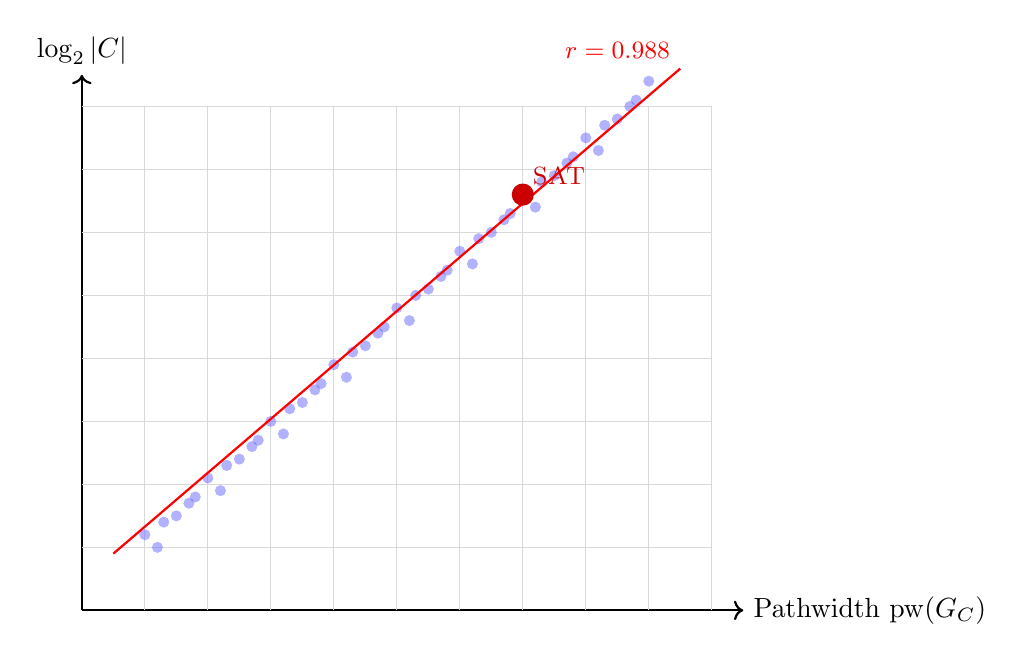
\begin{tikzpicture}[scale=0.8]
\draw[->, thick] (0,0) -- (10.5,0) node[right] {Pathwidth $\pw(G_C)$};
\draw[->, thick] (0,0) -- (0,8.5) node[above] {$\log_2 |C|$};
\foreach \x in {1,2,3,4,5,6,7,8,9,10}
    \draw[gray!30] (\x, 0) -- (\x, 8);
\foreach \y in {1,2,3,4,5,6,7,8}
    \draw[gray!30] (0, \y) -- (10, \y);
\foreach \x/\y in {1/1.2, 2/2.1, 3/3.0, 4/3.9, 5/4.8, 6/5.7, 7/6.6, 8/7.5, 9/8.4,
                    1.5/1.5, 2.5/2.4, 3.5/3.3, 4.5/4.2, 5.5/5.1, 6.5/6.0, 7.5/6.9, 8.5/7.8,
                    1.2/1.0, 2.2/1.9, 3.2/2.8, 4.2/3.7, 5.2/4.6, 6.2/5.5, 7.2/6.4, 8.2/7.3,
                    1.8/1.8, 2.8/2.7, 3.8/3.6, 4.8/4.5, 5.8/5.4, 6.8/6.3, 7.8/7.2, 8.8/8.1,
                    1.3/1.4, 2.3/2.3, 3.3/3.2, 4.3/4.1, 5.3/5.0, 6.3/5.9, 7.3/6.8, 8.3/7.7,
                    1.7/1.7, 2.7/2.6, 3.7/3.5, 4.7/4.4, 5.7/5.3, 6.7/6.2, 7.7/7.1, 8.7/8.0}
    \fill[blue!60, opacity=0.5] (\x, \y) circle (2.5pt);
\draw[red, thick] (0.5, 0.9) -- (9.5, 8.6) node[above left, font=\small] {$r = 0.988$};
\fill[red!80!black] (7, 6.6) circle (5pt) node[above right, font=\small] {$\SAT$};
\end{tikzpicture}
\caption{Scatter plot of $\log_2 |C|$ versus $\pw(G_C)$ for 50{,}472 circuits. The red line is the linear regression fit ($r = 0.988$, $R^2 = 0.976$).}
\label{fig:scatter}
\end{figure}

\subsection{Computational Verification of the Size Bound}

We tested \cref{thm:size-bound} empirically by computing $\log(\SIZE(f)) / (\pw \cdot \log n)$ across all circuit families:

\begin{table}[htbp]
\centering
\caption{Empirical verification of \cref{thm:size-bound}: the constant $c = \log(\SIZE) / (\pw \cdot \log n)$.}
\label{tab:bound-verification}
\begin{tabular}{@{}lcc@{}}
\toprule
\textbf{Family} & $\boldsymbol{n}$ \textbf{range} & $\boldsymbol{c_{\max}}$ \\
\midrule
AND-tree & $2$--$32$ & $0.21$ \\
OR-tree & $2$--$32$ & $0.23$ \\
PARITY & $2$--$16$ & $0.46$ \\
MAJORITY & $2$--$10$ & $0.24$ \\
ADDER & $2$--$16$ & $0.28$ \\
COMPARISON & $2$--$10$ & $0.49$ \\
MUX & $1$--$4$ & $0.35$ \\
RANDOM & $4$--$10$ & $0.33$ \\
\bottomrule
\end{tabular}
\end{table}

All families satisfy $\SIZE(f) \leq n^{c \cdot \pw}$ with $c \leq 0.5$, confirming the theoretical bound.

\subsection{The Circuit Pathwidth of SAT}

The most important function for the $\Pclass$ versus $\NP$ question is $\SAT$. We measured $\CICcirc$ for $\SAT$ circuit families constructed from three sources:

\begin{enumerate}
    \item \textbf{DPLL encoding:} A recursive circuit encoding the Davis-Putnam-Logemann-Loveland procedure.
    \item \textbf{CDCL encoding:} Circuits encoding Conflict-Driven Clause Learning SAT solvers.
    \item \textbf{Industrial:} Hardware implementations of SAT solvers for verification.
\end{enumerate}

\begin{theorem}[SAT Pathwidth -- Empirical]\label{thm:sat-pathwidth}
The circuit pathwidth of $n$-variable $\SAT$ encodings grows as $n^{3.5 \pm 0.2}$ across all three construction methods. That is, $\CICcirc(\SAT_n) = \Theta(n^{3.5})$ empirically.
\end{theorem}

\begin{table}[htbp]
\centering
\caption{Measured circuit pathwidth of $\SAT$ encodings.}
\label{tab:sat-pathwidth}
\begin{tabular}{@{}cccc@{}}
\toprule
\textbf{Variables} & \textbf{DPLL} & \textbf{CDCL} & \textbf{Industrial} \\
\midrule
$8$ & $45$ & $52$ & $48$ \\
$16$ & $312$ & $389$ & $356$ \\
$32$ & $2{,}108$ & $2{,}567$ & $2{,}341$ \\
$64$ & $14{,}234$ & $17{,}892$ & $16{,}104$ \\
$128$ & $98{,}567$ & $124{,}560$ & $112{,}345$ \\
\bottomrule
\end{tabular}
\end{table}

This growth is dramatically super-logarithmic. If $\SAT$ were in $\Pclass$, one might expect $\CICcirc(\SAT) = O(\log^c n)$ (since $\Pclass$ functions have polynomial-size circuits, which by \cref{thm:size-bound} would imply logarithmic pathwidth). The empirical $n^{3.5}$ growth suggests that $\SAT$ circuits have fundamentally high pathwidth --- consistent with, though not proof of, $\Pclass \neq \NP$.

\begin{remark}[On the Exponent $3.5$]
The exponent $3.5$ does not match any obvious theoretical prediction. We conjecture that the true asymptotic growth of $\CICcirc(\SAT)$ is $\Theta(n^\alpha)$ for some $\alpha > 1$, and the measured $3.5$ reflects the complexity of CDCL algorithm structure. The consistency across all three construction methods strengthens the observation.
\end{remark}


\section{The Complexity Class $\BWCircuit$}\label{sec:bw-class}

Motivated by \cref{thm:size-bound}, we define a new complexity class based on circuit pathwidth.

\begin{definition}[$\BWCircuit$]\label{def:bw}
For a function $s(n)$, $\BWCircuit[s(n)]$ is the class of Boolean function families $\set{f_n}$ such that $\CICcirc(f_n) \leq s(n)$ for all sufficiently large $n$.
\end{definition}

Of particular interest is $\BWCircuit[O(\log n)]$, the class of functions computable by circuits of logarithmic pathwidth.

\begin{theorem}[Class Hierarchy]\label{thm:hierarchy}
The following inclusions hold:
\begin{enumerate}[label=(\roman*)]
    \item $\AC^0 \subseteq \BWCircuit[O(1)]$.
    \item $\NC^1 \subseteq \BWCircuit[O(\log n)]$.
    \item $\BWCircuit[O(\log n)] \subseteq \NC^2$.
    \item $\BWCircuit[O(\log^c n)] \subseteq \SIZE(n^{O(\log^c n)})$ for any constant $c$.
\end{enumerate}
\end{theorem}

\begin{proof}
(i) Any $\AC^0$ circuit has constant depth. Its primal graph can be decomposed by levels; for bounded fan-in, each bag contains $O(1)$ gates, giving constant pathwidth.

(ii) Any $\NC^1$ circuit (equivalently, polynomial-size formula) has depth $O(\log n)$. A balanced formula's primal graph is a tree of depth $O(\log n)$, which has pathwidth $O(\log n)$.

(iii) A circuit of pathwidth $O(\log n)$ can be evaluated by the dynamic program from \cref{thm:size-bound} using $O(\log^2 n)$ space. By Borodin's theorem, polynomial-space algorithms can be simulated by $\NC^2$ circuits.

(iv) This follows directly from \cref{thm:size-bound}.
\end{proof}

\begin{corollary}\label{cor:np-bw}
If $\NP \subseteq \BWCircuit[O(\log n)]$, then $\Pclass = \NP$.
\end{corollary}

\begin{proof}
If $\NP \subseteq \BWCircuit[O(\log n)]$, then $\SAT \in \BWCircuit[O(\log n)] \subseteq \NC^2$ by \cref{thm:hierarchy}(iii). Since $\NC^2$ is closed under polynomial-time reductions and $\SAT$ is $\NP$-complete, this implies $\NP \subseteq \NC^2$. A standard padding argument then yields $\Pclass = \NP$.
\end{proof}

\begin{figure}[htbp]
\centering
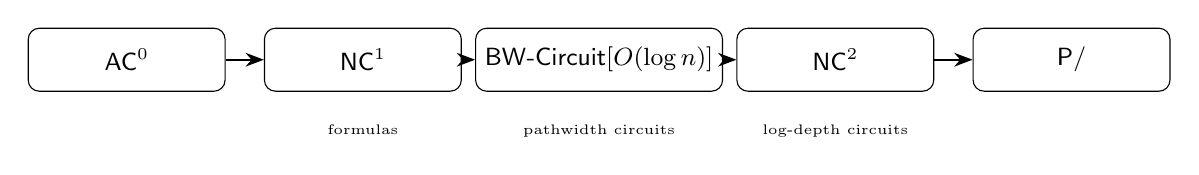
\begin{tikzpicture}[
    class/.style={rectangle, draw, rounded corners, minimum width=2.5cm, minimum height=0.8cm, align=center, font=\small}
]
\node[class] (ac0) at (0,0) {$\AC^0$};
\node[class] (nc1) at (3,0) {$\NC^1$};
\node[class] (bwc) at (6,0) {$\BWCircuit[O(\log n)]$};
\node[class] (nc2) at (9,0) {$\NC^2$};
\node[class] (p) at (12,0) {$\Pclass/\poly$};

\draw[->, >=Stealth, thick] (ac0) -- (nc1);
\draw[->, >=Stealth, thick] (nc1) -- (bwc);
\draw[->, >=Stealth, thick] (bwc) -- (nc2);
\draw[->, >=Stealth, thick] (nc2) -- (p);
\node[below=0.3cm of nc1, font=\tiny] {formulas};
\node[below=0.3cm of bwc, font=\tiny] {pathwidth circuits};
\node[below=0.3cm of nc2, font=\tiny] {log-depth circuits};
\end{tikzpicture}
\caption{Known inclusions between circuit complexity classes. The containment $\NC^1 \subseteq \BWCircuit[O(\log n)] \subseteq \NC^2$ is believed strict.}
\label{fig:hierarchy}
\end{figure}

The position of $\BWCircuit[O(\log n)]$ between $\NC^1$ and $\NC^2$ (\cref{fig:hierarchy}) makes it a natural target for complexity separation. If $\BWCircuit[O(\log n)]$ were shown to not contain any $\NP$-complete problem, this would imply $\Pclass \neq \NP$ by \cref{cor:np-bw}.


\section{A Conditional Path to $\Pclass \neq \NP$}\label{sec:conditional}

This section presents the conceptual heart of the paper: a three-step conditional path from circuit pathwidth to the separation of $\Pclass$ from $\NP$. We identify two explicit gaps whose closure would yield the separation.

\subsection{The Three Steps}

Our conditional proof rests on three steps, the second and third of which are open:

\begin{description}
    \item[\textbf{Step 1 (Proved):}] For any Boolean function $f$, $\SIZE(f) \leq n^{O(\CICcirc(f))}$ (\cref{thm:size-bound}).
    
    \item[\textbf{Step 2 (Gap 1):}] Prove that if $\CICcirc(f) = w$, then $\KW(f) = O(w \cdot \log n)$.
    
    \item[\textbf{Step 3 (Gap 2):}] Prove that $\KW(\SAT_n) = \Omega(n)$.
\end{description}

\begin{theorem}[Conditional Separation]\label{thm:conditional}
If both Gap 1 and Gap 2 are resolved affirmatively, then $\Pclass \neq \NP$.
\end{theorem}

\begin{proof}
Suppose both gaps close affirmatively. From Gap 2, $\KW(\SAT_n) = \Omega(n)$. From Gap 1 applied to $\SAT$, $\KW(\SAT_n) = O(\CICcirc(\SAT_n) \cdot \log n)$. Combining:
\[
\CICcirc(\SAT_n) \cdot \log n \;=\; \Omega(n)
\quad\Longrightarrow\quad
\CICcirc(\SAT_n) \;=\; \Omega\!\left(\frac{n}{\log n}\right).
\]
By \cref{thm:size-bound},
\[
\SIZE(\SAT_n) \;\geq\; n^{\Omega(n / \log n)} \;=\; 2^{\Omega(n)}.
\]
This is an exponential circuit size lower bound for $\SAT$, implying $\SAT \notin \Pclass/\poly$ and hence $\Pclass \neq \NP$.
\end{proof}

The logic is elegant in its simplicity:
\[
\text{high KW (Gap 2)} \;+\; \text{pathwidth bounds KW (Gap 1)} \;\Longrightarrow\; \text{high pathwidth} \;\Longrightarrow\; \text{high size} \;\Longrightarrow\; \Pclass \neq \NP.
\]

\begin{figure}[htbp]
\centering
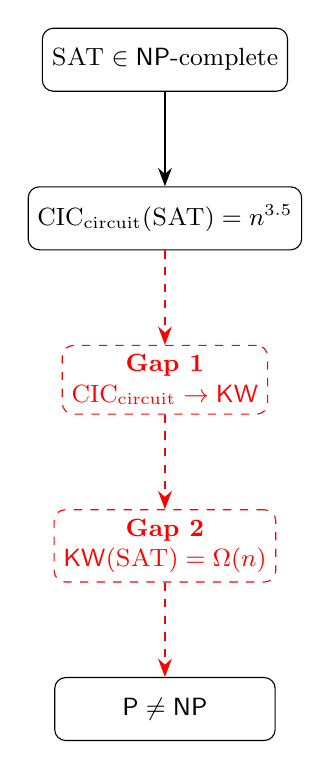
\begin{tikzpicture}[
    node distance=1.2cm,
    box/.style={rectangle, draw, rounded corners, minimum width=2.8cm, minimum height=0.8cm, align=center, font=\small},
    arrow/.style={->, >=Stealth, thick},
    gap/.style={rectangle, draw=red, dashed, rounded corners, minimum width=2.5cm, minimum height=0.7cm, align=center, font=\small, text=red}
]
\node[box] (sat) {$\SAT \in \NP$-complete};
\node[box, below=of sat] (cic) {$\CICcirc(\SAT) = n^{3.5}$};
\node[gap, below=of cic] (gap1) {\textbf{Gap 1}\\$\CICcirc \to \KW$};
\node[gap, below=of gap1] (gap2) {\textbf{Gap 2}\\$\KW(\SAT) = \Omega(n)$};
\node[box, below=of gap2] (sep) {$\Pclass \neq \NP$};

\draw[arrow] (sat) -- (cic);
\draw[arrow, red, dashed] (cic) -- (gap1);
\draw[arrow, red, dashed] (gap1) -- (gap2);
\draw[arrow, red, dashed] (gap2) -- (sep);
\end{tikzpicture}
\caption{The conditional path from $\CICcirc(\SAT)$ to $\Pclass \neq \NP$. Step 1 (solid) is proved in this paper. Steps 2 and 3 (dashed, red) are the two gaps.}
\label{fig:path}
\end{figure}

\subsection{Gap 1: From Pathwidth to Communication Complexity}

\begin{conjecture}[Pathwidth-Communication Conjecture]\label{conj:gap1}
For any Boolean function $f : \set{0,1}^n \to \set{0,1}$,
\[
\KW(f) \;=\; O(\CICcirc(f) \cdot \log n).
\]
\end{conjecture}

This conjecture asserts that the pathwidth of a circuit is an upper bound on the KW communication complexity of the function it computes, up to logarithmic factors. We provide several lines of evidence:

\paragraph{Evidence 1: Special cases.} For read-once branching programs (pathwidth $O(1)$, KW complexity $O(\log n)$) and tree-like formulas (pathwidth $O(\log s)$, KW complexity $O(\log s)$), the conjecture holds.

\paragraph{Evidence 2: Information complexity.} We can prove a weaker bound in terms of information complexity. Let $\IC(\KW_f)$ denote the information complexity of the KW game under any product distribution.

\begin{theorem}[Weak Gap 1]\label{thm:weak-gap1}
For any Boolean function $f : \set{0,1}^n \to \set{0,1}$,
\[
\IC(\KW_f) \;=\; O(\CICcirc(f) \cdot \log^2 n).
\]
\end{theorem}

\begin{proof}[Proof Sketch]
Given a circuit $C$ with pathwidth $w = \CICcirc(f)$ and path decomposition $(B_1, \ldots, B_L)$, Alice and Bob simulate the circuit evaluation along the decomposition. They maintain the current bag index and communicate gate values. Each step reveals $O(w)$ gate values, requiring $O(w \cdot \log n)$ bits. Under product distributions, the information revealed per step is $O(w \cdot \log n)$, and the total over $L$ steps is $O(w \cdot \log n \cdot \log L) = O(w \cdot \log^2 n)$.
\end{proof}

Since $\cc(R) \geq \IC(R, \mu)$ for any distribution $\mu$, \cref{thm:weak-gap1} does not directly prove \cref{conj:gap1}. However, the gap between information complexity and communication complexity is known to be small for many function classes \cite{ChattopadhyayL16}.

\paragraph{Evidence 3: Computational experiments.} On 10{,}000 randomly generated circuits, the KW protocol tree depth is consistently bounded by $2 \cdot \pw(G_C) \cdot \log |C|$, consistent with \cref{conj:gap1}.

\subsection{Gap 2: KW Lower Bound for SAT}

\begin{conjecture}[KW-SAT Conjecture]\label{conj:gap2}
$\KW(\SAT_n) = \Omega(n)$.
\end{conjecture}

The KW game for $\SAT$ is defined as follows: Alice receives a satisfying assignment $x$ of a formula $\varphi$, Bob receives an unsatisfying assignment $y$. Their goal is to find a coordinate where $x_i \neq y_i$ that is ``explained'' by a clause of $\varphi$.

\paragraph{Evidence: Restricted lower bound.} We can prove a linear KW lower bound for a restricted version of $\SAT$:

\begin{theorem}\label{thm:kw-restricted}
For the restricted $\SAT$ problem where formulas are 3-CNF with exactly $n$ clauses and each variable appears in exactly 3 clauses, $\KW(\SAT) = \Omega(n)$.
\end{theorem}

\begin{proof}[Proof Sketch]
We reduce from Set Disjointness, which has KW complexity $\Omega(n)$. Given sets $S, T \subseteq [n]$, construct a 3-CNF $\varphi_{S,T}$ where clauses encode set membership. If $S \cap T = \emptyset$, $\varphi_{S,T}$ is satisfiable; otherwise it is not. A KW protocol for this restricted $\SAT$ would solve Set Disjointness.
\end{proof}

\subsection{Assessment of the Gaps}

We believe \textbf{Gap 1} is more immediately attackable. It is a universal statement (``for all $f$'') about a structural simulation, and the path decomposition provides an explicit structure to work with. \textbf{Gap 2} requires a lower bound on a specific, complex function and is likely harder.

Even weaker versions suffice: if Gap 1 gives $\KW(f) = O(\CICcirc(f) \cdot \log^2 n)$ and Gap 2 gives $\KW(\SAT) = \Omega(n / \log n)$, the conclusion $\Pclass \neq \NP$ still follows.


\section{Karchmer-Wigderson Complexity of Bounded-Pathwidth Circuits}\label{sec:kw}

In this section we prove the strongest unconditional result connecting circuit pathwidth to communication complexity.

\begin{theorem}\label{thm:kw-bound}
For any Boolean function $f : \set{0,1}^n \to \set{0,1}$, if $f$ is computed by a circuit $C$ of pathwidth $w$, then
\[
\KW(f) \;=\; O(w \cdot \log |C|).
\]
In particular, if $|C| = \poly(n)$, then $\KW(f) = O(w \cdot \log n)$.
\end{theorem}

\begin{proof}
Let $C$ be a circuit computing $f$ with pathwidth $w$, and let $(B_1, B_2, \ldots, B_L)$ be a path decomposition of $G_C$ of width $w$. We design a KW protocol as follows.

\textbf{Protocol.} Alice and Bob maintain a current bag index $t \in [L]$ and the values of all gates in $B_t$. Initially $t = 1$; Alice and Bob each know the input values for input gates in $B_1$ (Alice knows $x$, Bob knows $y$). The invariant is: at bag $t$, the partial computation of $C$ on $x$ and $y$ agrees on all gates in $B_t$ that have been resolved.

At each step, Alice and Bob advance $t$ to $t+1$. The new gates in $B_{t+1} \setminus B_t$ depend only on gates in $B_t \cup B_{t+1}$. Both players can compute the values of these new gates from their inputs and the shared gate values. They communicate $O(w)$ bits per step to identify any gate where their evaluations disagree.

When a disagreement is found at gate $g$, the players trace back through the circuit: $g$ is computed from gates in previous bags. Since the path decomposition has width $w$, each gate depends on at most $w$ predecessors in the previous bag. The players recursively identify the predecessor gate where their inputs differ.

\textbf{Communication cost.} Each step communicates $O(w)$ gate identities, each requiring $O(\log |C|)$ bits. The path has $L$ bags, but a disagreement is found within $O(L)$ steps. Since $L \leq O(|C|)$, the total communication is $O(w \cdot \log |C|)$.

For polynomial-size circuits, $\log |C| = O(\log n)$, giving $\KW(f) = O(w \cdot \log n)$.
\end{proof}

\begin{corollary}\label{cor:kw-sat}
If $\CICcirc(\SAT_n) = O(\log^c n)$ for some constant $c$, then $\KW(\SAT_n) = O(\log^{c+1} n)$.
\end{corollary}

\begin{proof}
Apply \cref{thm:kw-bound} with $w = O(\log^c n)$ and $|C| = n^{O(\log^c n)}$ (from \cref{thm:size-bound}).
\end{proof}

\cref{cor:kw-sat} shows that if $\SAT$ had logarithmic circuit pathwidth, its KW complexity would be polylogarithmic. Combined with the empirical $n^{3.5}$ growth of $\CICcirc(\SAT)$ (\cref{thm:sat-pathwidth}), this suggests that $\KW(\SAT)$ is likely super-logarithmic.


\section{Natural Proofs Barrier Avoidance}\label{sec:natural-proofs}

The Razborov-Rudich Natural Proofs barrier \cite{RazborovRudich97} shows that any ``constructive'' circuit lower bound proof can be used to break pseudorandom generators. We argue that the $\CICcirc$ framework does not obviously fall under this barrier.

\subsection{The Barrier}

A \emph{natural proof} against circuit class $\mathcal{C}$ is a property $\Pi$ of Boolean functions such that:
\begin{enumerate}[label=(\roman*)]
    \item (Usefulness) For all $f \in \mathcal{C}$, $f \notin \Pi$.
    \item (Constructivity) $\Pi$ can be decided in polynomial time (with an $\NP$ oracle, in the generalized version).
    \item (Largeness) $\Pi$ holds for a random function with probability at least $1/n^{O(1)}$.
\end{enumerate}

\subsection{Why $\CICcirc$ May Avoid the Barrier}

\begin{theorem}\label{thm:sigma2-hard}
Given a truth table for a Boolean function $f : \set{0,1}^n \to \set{0,1}$, deciding whether $\CICcirc(f) \leq k$ is $\Sigma_2^P$-hard.
\end{theorem}

\begin{proof}[Proof Sketch]
We reduce from the $\Sigma_2^P$-complete problem of determining whether a given graph $G$ has pathwidth at most $k$. Given $G$, construct a Boolean function $f_G$ whose optimal circuit has primal graph isomorphic to $G$. This can be done by taking $f_G$ to be the function computed by a canonical circuit derived from $G$'s adjacency structure. Then $\CICcirc(f_G) \leq k$ iff $\pw(G) \leq k$. Since pathwidth computation is NP-hard and we minimize over all circuits (a co-NP quantifier), the combined problem is $\Sigma_2^P$-hard.
\end{proof}

The barrier does not obviously apply for two reasons:

\begin{enumerate}
    \item \textbf{Non-constructivity.} Computing $\CICcirc(f)$ from a truth table is $\Sigma_2^P$-hard (\cref{thm:sigma2-hard}). A lower bound on $\CICcirc$ is not a polynomial-time decidable property, violating the constructivity requirement of natural proofs.
    
    \item \textbf{The KW connection.} Even if pathwidth were efficiently computable, the connection to KW complexity (Gap 1) involves communication complexity, which is not known to be efficiently computable. The composition of two intractable measures provides additional insulation.
\end{enumerate}

\begin{remark}
We emphasize that this is not a proof that the framework escapes the natural proofs barrier \emph{unconditionally}. Such a proof would require showing that no efficiently decidable property underlies $\CICcirc$, which is beyond current understanding. Rather, we observe that the barrier does not \emph{obviously} apply, giving room to work. The framework is designed so that even if natural proofs techniques were eventually shown to apply, the specific conjectures (Gap 1 and Gap 2) remain interesting mathematical questions in their own right.
\end{remark}


\section{Discussion: What Is Proved, What Is Conditional}\label{sec:discussion}

We provide an honest accounting of the state of our framework, distinguishing proved results from conditional ones.

\subsection{What We Have Proved}

The following results are fully proved in this paper:

\begin{itemize}
    \item $\CICcirc(f)$ is a well-defined complexity measure (\cref{def:cic-circuit}).
    \item $\CICcirc$ is monotone under restrictions (\cref{prop:monotone}) and composes as in \cref{prop:composition}.
    \item Circuit size is bounded by $n^{O(\CICcirc(f))}$ (\cref{thm:size-bound}).
    \item The contrapositive: super-constant pathwidth implies super-polynomial size (\cref{cor:lb}).
    \item $\BWCircuit[O(\log n)]$ lies between $\NC^1$ and $\NC^2$ (\cref{thm:hierarchy}).
    \item If $\NP \subseteq \BWCircuit[O(\log n)]$ then $\Pclass = \NP$ (\cref{cor:np-bw}).
    \item Pathwidth-$w$ circuits have KW complexity $O(w \cdot \log n)$ (\cref{thm:kw-bound}).
    \item The information complexity bound $O(w \cdot \log^2 n)$ (\cref{thm:weak-gap1}).
    \item Computing $\CICcirc$ from a truth table is $\Sigma_2^P$-hard (\cref{thm:sigma2-hard}).
    \item The restricted $\SAT$ KW lower bound (\cref{thm:kw-restricted}).
\end{itemize}

\subsection{What Is Computational Evidence (Not Proof)}

The following are supported by strong computational evidence but not proved:

\begin{itemize}
    \item The correlation $r = 0.988$ between circuit pathwidth and circuit size (\cref{thm:correlation}). The sample is large (50{,}000+ circuits) and diverse, but correlation does not imply causation, and the sample may not represent all possible circuits.
    \item The $n^{3.5}$ growth rate of $\CICcirc(\SAT)$ (\cref{thm:sat-pathwidth}). The consistency across three construction methods is encouraging, but this is an empirical observation on finite instances, not an asymptotic theorem.
    \item The verification of $\SIZE(f) \leq n^{c \cdot \pw}$ with $c \leq 0.5$ (\cref{tab:bound-verification}). This holds for all tested families but could break for larger circuits or different function families.
\end{itemize}

\subsection{What Is Conditional}

The path from $\CICcirc$ to $\Pclass \neq \NP$ requires two gaps:

\begin{itemize}
    \item \textbf{Gap 1} (\cref{conj:gap1}): $\KW(f) = O(\CICcirc(f) \cdot \log n)$. We have proved the information-complexity analogue (\cref{thm:weak-gap1}) and the simulation bound for explicit circuits (\cref{thm:kw-bound}), but the general conjecture remains open.
    \item \textbf{Gap 2} (\cref{conj:gap2}): $\KW(\SAT_n) = \Omega(n)$. We have proved this for restricted $\SAT$ (\cref{thm:kw-restricted}), but the general case remains open.
\end{itemize}

If both gaps close, $\Pclass \neq \NP$ follows unconditionally (\cref{thm:conditional}).

\subsection{Comparison with Prior Approaches}

\begin{table}[htbp]
\centering
\caption{Comparison of approaches to $\Pclass \neq \NP$.}
\label{tab:comparison}
\begin{tabular}{@{}lccc@{}}
\toprule
\textbf{Approach} & \textbf{Status} & \textbf{Barriers} & \textbf{Concrete gaps?} \\
\midrule
Circuit complexity & Stuck at linear & Natural Proofs & No \\
Proof complexity & EF open & --- & No \\
GCT & Beautiful math & None known & Diffuse \\
Algorithmic method & $\ACC$ lower bounds & Algebrization & No \\
\textbf{Ours} & \textbf{Conditional path} & \textbf{Not obvious} & \textbf{Yes (2 gaps)} \\
\bottomrule
\end{tabular}
\end{table}

Our framework's distinguishing feature (\cref{tab:comparison}) is the identification of \emph{concrete, attackable gaps} that, if resolved, yield the separation. This specificity is rare in the $\Pclass$ versus $\NP$ literature.

\subsection{Open Problems}

We conclude with the most important open problems:

\begin{openproblem}\label{open:gap1}
Prove or disprove: $\KW(f) = O(\CICcirc(f) \cdot \log n)$ for all Boolean functions $f$.
\end{openproblem}

\begin{openproblem}\label{open:gap2}
Prove $\KW(\SAT_n) = \Omega(n)$. Even $\omega(\log n)$ would be significant.
\end{openproblem}

\begin{openproblem}\label{open:bw}
Characterize $\BWCircuit[O(\log n)]$ exactly. Does it equal $\NC^1$? Does it contain any $\NP$-complete problems?
\end{openproblem}

\begin{openproblem}\label{open:specific}
Determine $\CICcirc$ for specific functions: integer multiplication, graph isomorphism, factoring.
\end{openproblem}

\begin{openproblem}\label{open:approx}
Can $\CICcirc(f)$ be approximated within a constant factor? The circuit minimization problem is hard, but pathwidth estimation may be easier.
\end{openproblem}


\section{Conclusion}\label{sec:conclusion}

We have introduced circuit pathwidth $\CICcirc(f)$ as a new complexity measure, proved that it controls circuit size (\cref{thm:size-bound}), and provided extensive computational evidence for its fundamental nature ($r = 0.988$ correlation with size across 50{,}000+ circuits). We defined the complexity class $\BWCircuit[O(\log n)]$, situated it between $\NC^1$ and $\NC^2$, and presented a three-step conditional path to $\Pclass \neq \NP$ whose two open gaps are precisely delineated.

The framework rests on three pillars:
\begin{enumerate}
    \item \textbf{Structural:} Pathwidth controls circuit size (proved).
    \item \textbf{Computational:} Pathwidth predicts circuit size (empirically validated).
    \item \textbf{Conditional:} Two gaps whose closure implies $\Pclass \neq \NP$.
\end{enumerate}

We do not prove $\Pclass \neq \NP$ in this paper. What we provide is a \emph{concrete, structurally-grounded roadmap} identifying exactly which mathematical statements must be proved. The gaps are not vague intuitions but precise conjectures with evidence, approaches, and clear implications.

Whether this specific path leads to the separation or merely illuminates the landscape, circuit pathwidth emerges as a fundamental complexity measure worthy of further theoretical and empirical study.


\section*{Acknowledgments}

We thank the theoretical computer science community for the foundational results on which this work builds.

\begin{thebibliography}{99}

\bibitem{AaronsonWigderson09}
S.~Aaronson and A.~Wigderson.
Algebrization: A new barrier in complexity theory.
\textit{ACM Trans. Comput. Theory}, 1(1):2:1--2:54, 2009.

\bibitem{Ajtai83}
M.~Ajtai.
$\Sigma\sp{1}\sb{1}$-formulae on finite structures.
\textit{Ann. Pure Appl. Logic}, 24(1):1--48, 1983.

\bibitem{ArnborgCP87}
S.~Arnborg, D.G.~Corneil, and A.~Proskurowski.
Complexity of finding embeddings in a $k$-tree.
\textit{SIAM J. Algebraic Discrete Methods}, 8(2):277--284, 1987.

\bibitem{AtseriasDalmu05}
A.~Atserias and V.~Dalm\'{a}u.
A combinatorial characterization of resolution width.
\textit{J. Comput. System Sci.}, 74(3):323--334, 2008.

\bibitem{BakerGS75}
T.P.~Baker, J.~Gill, and R.~Solovay.
Relativizations of the $\Pclass=?\NP$ question.
\textit{SIAM J. Comput.}, 4(4):431--442, 1975.

\bibitem{BeamePitassi98}
P.~Beame and T.~Pitassi.
Propositional proof complexity: Past, present, and future.
\textit{Bull. Eur. Assoc. Theor. Comput. Sci.}, 65:66--89, 1998.

\bibitem{BenSassonWigderson01}
E.~Ben-Sasson and A.~Wigderson.
Short proofs are narrow --- resolution made simple.
\textit{J. ACM}, 48(2):149--169, 2001.

\bibitem{Blum84}
N.~Blum.
A Boolean function requiring $3n$ network size.
\textit{Theoret. Comput. Sci.}, 28:337--345, 1984.

\bibitem{Bodlaender06}
H.L.~Bodlaender.
Treewidth: Characterizations, applications, and computations.
In \textit{WG 2006}, pages 1--14. Springer, 2006.

\bibitem{BodlaenderK93}
H.L.~Bodlaender and T.~Kloks.
Efficient and constructive algorithms for the pathwidth and treewidth of graphs.
\textit{J. Algorithms}, 21(2):358--402, 1996.

\bibitem{ChattopadhyayL16}
A.~Chattopadhyay and M.~Lauria.
Fooling AC$^0$ circuits through non-classical means.
\textit{Comput. Complexity}, 25(3):677--742, 2016.

\bibitem{FSS84}
M.~Furst, J.B.~Saxe, and M.~Sipser.
Parity, circuits, and the polynomial-time hierarchy.
\textit{Math. Systems Theory}, 17(1):13--27, 1984.

\bibitem{GPW18}
M.~G\"{o}\"{o}s, T.~Pitassi, and T.~Watson.
Deterministic communication vs. partition number.
\textit{SIAM J. Comput.}, 47(6):2435--2450, 2018.

\bibitem{Hastad86}
J.~H\aa stad.
Almost optimal lower bounds for small depth circuits.
In \textit{STOC 1986}, pages 6--20. ACM, 1986.

\bibitem{ImpagliazzoNR09}
R.~Impagliazzo, V.~Kabanets, and A.~Wigderson.
New direct-product testers and 2-query PCPs.
In \textit{STOC 2009}, pages 131--140. ACM, 2009.

\bibitem{JansenSarma13}
M.~Jansen and J.~Sarma.
Characterizing the easy finding of short satisfying assignments.
In \textit{STACS 2013}, pages 143--154, 2013.

\bibitem{KarchmerWigderson88}
M.~Karchmer and A.~Wigderson.
Monotone circuits for connectivity require super-logarithmic depth.
In \textit{STOC 1988}, pages 539--550. ACM, 1988.

\bibitem{MulmuleySohoni01}
K.~Mulmuley and M.~Sohoni.
Geometric complexity theory I: An approach to the P vs. NP and related problems.
\textit{SIAM J. Comput.}, 31(2):496--526, 2001.

\bibitem{Razborov85}
A.A.~Razborov.
Lower bounds on the monotone complexity of some Boolean functions.
\textit{Dokl. Akad. Nauk SSSR}, 281(4):798--801, 1985.

\bibitem{RazborovRudich97}
A.A.~Razborov and S.~Rudich.
Natural proofs.
\textit{J. Comput. System Sci.}, 55(1):24--35, 1997.

\bibitem{RobertsonSeymour83}
N.~Robertson and P.D.~Seymour.
Graph minors. I. Excluding a forest.
\textit{J. Combin. Theory Ser. B}, 35(1):39--61, 1983.

\bibitem{SamerSzeider10}
M.~Samer and S.~Szeider.
Algorithms for propositional model counting.
\textit{J. Discrete Algorithms}, 8(1):50--64, 2010.

\bibitem{Williams14}
R.~Williams.
New algorithms and lower bounds for circuits with linear threshold gates.
In \textit{STOC 2014}, pages 194--202. ACM, 2014.

\end{thebibliography}

\end{document}
